\documentclass[11pt,a4paper]{article}
\usepackage[top=1.2cm, bottom=1.8cm, left=1.8cm, right=1.8cm]{geometry}

\usepackage{float}
\usepackage{subfig}
\usepackage{graphicx}
\usepackage{xcolor}
\usepackage[utf8]{inputenc}
\usepackage{enumitem}
\usepackage{siunitx}
\usepackage[newfloat]{minted}
\usepackage{caption}
\usepackage{amsmath}
\usepackage{amsfonts,amssymb}
\usepackage[makeroom]{cancel}

% Declarations for tikz drawings
\usepackage{tikz}
\usepackage{pgfplots}
\usetikzlibrary{calc}
\definecolor{lightgreen}{HTML}{90EE90}
\newcommand*{\boxcolor}{lightgreen}
\makeatletter
\renewcommand{\boxed}[1]{\textcolor{\boxcolor}{%
\tikz[baseline={([yshift=-1ex]current bounding box.center)}] \node [rectangle, minimum width=5ex,rounded corners,draw,line width=0.25mm] {\normalcolor\m@th$\displaystyle#1$};}}
 \makeatother

 % Fix for symbol errors in code listings (see https://tex.stackexchange.com/a/343506)
 \usepackage{etoolbox,xpatch}
 \makeatletter
 \AtBeginEnvironment{minted}{\dontdofcolorbox}
 \def\dontdofcolorbox{\renewcommand\fcolorbox[4][]{##4}}
 \xpatchcmd{\inputminted}{\minted@fvset}{\minted@fvset\dontdofcolorbox}{}{}
 \xpatchcmd{\mintinline}{\minted@fvset}{\minted@fvset\dontdofcolorbox}{}{}
 \makeatother
 % Fix for distance of captions from listings
 \captionsetup[listing]{skip=-10pt}

% \usepackage[style=authoryear, backend=biber]{biblatex}
% \addbibresource{main.bib}
\DeclareMathOperator*{\argmin}{arg\,min}
\DeclareMathOperator*{\argmax}{arg\,max}

\title{COMP6248: Lab Exercise 8}
\author{
David Jones (dsj1n15@soton.ac.uk)}
\date{}
\setlength{\intextsep}{1mm}

\definecolor{mintedbackground}{rgb}{0.95,0.95,0.95}
\newmintedfile[pythoncode]{python}{
    bgcolor=mintedbackground,
    style=friendly,
    % fontfamily=fi4,
    fontsize=\small,
    linenos=true,
    numberblanklines=true,
    numbersep=5pt,
    gobble=0,
    frame=leftline,
    framerule=0.4pt,
    framesep=2mm,
    funcnamehighlighting=true,
    tabsize=4,
    obeytabs=false,
    mathescape=false
    samepage=false,
    showspaces=false,
    showtabs =false,
    texcl=false,
}

\newcommand{\norm}[1]{\left\lVert#1\right\rVert}

\begin{document}

\maketitle
\textbf{Task:} Exploring Latent Spaces
\vspace{-0.5em}
\section{Exercise 1 \& 2}
% \textbf{Exercise 1.1:} Systematically Sampling a VAE
Systematically sampling of the 2D latent space of an Variational Autoencoder (VAE) and Autoencoder (AE) across $z= -4\enskip \text{to}\enskip 4$ for both dimensions. Top left: (-4, 4). Note that the AE architecture is expanded from the original lab to include a dense hidden layer (ReLU activation) for both encoding and decoding; this was required to reduce artefacts in reconstructions.  \\

\begin{figure}[H]
    \centering
    \begin{tabular}{ccc}
    \subfloat[VAE (Ex 1)]{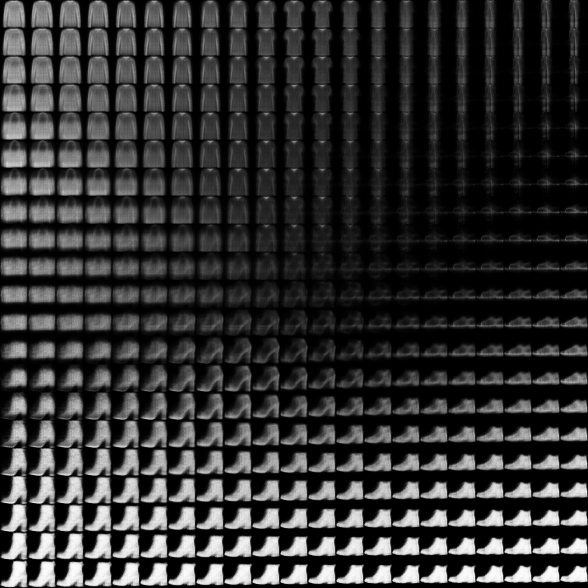
\includegraphics[width=3.5in]{figures/vae_sample.png}}
    \hspace{0.5em}
    \subfloat[AE (Ex 2)]{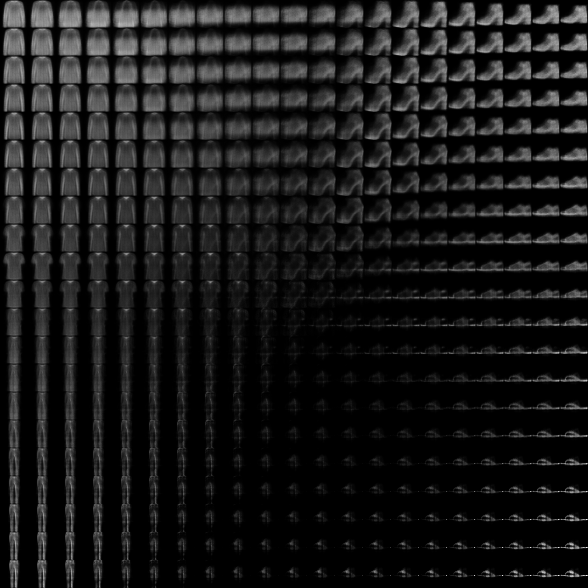
\includegraphics[width=3.5in]{figures/ae_sample.png}}
    \end{tabular}
    \caption{Latent space sampling trained on the Fashion-MNIST dataset.}
    \label{fig:pca_sg}
\end{figure}

\noindent At first glance, sampling from both models has resulted in images like those originally in the Fashion-MNIST dataset. However, there are notable differences in generation capability of each model. The VAE has smooth transitions between samples that are close in the latent space; often incorporating features from multiple items in the original dataset, e.g. heeled boots. The AE has no formal structure dictated and therefore does not need to ensure that two close points give a similar result; this typically leads to larger differences between items. Additionally, the AE is not regularised to always give a meaningful result; this has occurred in the example (bottom-middle).


\end{document}

